% template adapted from https://github.com/jgm/pandoc-templates/blob/master/default.latex
%%%%%%%%%%%%%%%%%%%%%%%%%%%%%%%%%%%%%%%%%%%%%%%%%%%%%%%%%%%%%%%%%%%%%%%%%%%%%%%%%%%%%%%%%

% Options for packages loaded elsewhere
\PassOptionsToPackage{unicode=true}{hyperref}
\PassOptionsToPackage{hyphens}{url}
  \PassOptionsToPackage{dvipsnames,svgnames*,x11names*}{xcolor}


\documentclass[
  11pt,
  french,
  A4paper,
  extrafontsizes,onecolumn,openright
  ]{memoir}

% Font family: lmodern by default
  \usepackage{lmodern}

% Double (or whatever) spacing

\usepackage{amssymb, amsmath}
\usepackage{ifxetex,ifluatex}
\usepackage{fixltx2e} % provides \textsubscript

% mathspec: arbitrary math fonts
  \usepackage{unicode-math}
\defaultfontfeatures{Ligatures=TeX,Scale=MatchLowercase}

% More font families
% Main font
% Specific sanserif font
% Specific monotype font
% Specific math font
% Chinese, Japanese, Corean fonts

% Use upquote if available, for straight quotes in verbatim environments
\IfFileExists{upquote.sty}{\usepackage{upquote}}{}
% Use microtype if available
\IfFileExists{microtype.sty}{%
\usepackage[]{microtype}
\UseMicrotypeSet[protrusion]{basicmath} % disable protrusion for tt fonts
}{}

% Verbatim in note

\usepackage{xcolor}

\usepackage{hyperref}
\hypersetup{
            pdftitle={Trajectoires de biodiversité en forêt tropicale exploitée},
            pdfauthor={Ariane Mirabel},
            pdfkeywords={Keyword in English, As a list},
            colorlinks=true,
            linkcolor=Maroon,
            citecolor=Blue,
            urlcolor=Blue,
            breaklinks=true}

% Don't use monospace font for urls
\urlstyle{same}


% Geometry package

% Listings package



% Tables
  \usepackage{longtable,booktabs}
  % Fix footnotes in tables (requires footnote package)
  \IfFileExists{footnote.sty}{\usepackage{footnote}\makesavenoteenv{longtable}}{}

% Graphics
  \usepackage{graphicx,grffile}
  \graphicspath{{images/}}
  \makeatletter
  \def\maxwidth{\ifdim\Gin@nat@width>\linewidth\linewidth\else\Gin@nat@width\fi}
  \def\maxheight{\ifdim\Gin@nat@height>\textheight\textheight\else\Gin@nat@height\fi}
  \makeatother
  % Scale images if necessary, so that they will not overflow the page
  % margins by default, and it is still possible to overwrite the defaults
  % using explicit options in \includegraphics[width, height, ...]{}
  \setkeys{Gin}{width=\maxwidth,height=\maxheight,keepaspectratio}



\setlength{\emergencystretch}{3em}  % prevent overfull lines
\providecommand{\tightlist}{%
  \setlength{\itemsep}{0pt}\setlength{\parskip}{0pt}}

  \setcounter{secnumdepth}{5}

% set default figure placement to htbp
\makeatletter
\def\fps@figure{htbp}
\makeatother

% Include headers (preamble.tex) here
%%% Complete the preamble of the LaTeX template
%%%------------------------------------------------------------------------------

%%% PACKAGES 
\usepackage{lipsum} % Dummy text.

\usepackage{enumitem}

  % load polyglossia as late as possible as it *could* call bidi if RTL lang (e.g. Hebrew or Arabic)
  \usepackage{polyglossia}
  \setmainlanguage[]{french}
  \setotherlanguage[variant=american]{english}
  \setotherlanguage[variant=british]{english}
  \setotherlanguage[]{french}




\usepackage[style=authoryear-ibid,backend=bibtex,citestyle=verbose-inote,pageref=true,isbn=false,backref=true,giveninits=true,uniquename=init,maxcitenames=2,maxbibnames=150,sorting=nyt,sortcites=false]{biblatex}
\addbibresource{MyBook.bib}
\addbibresource{packages.bib}
\addbibresource{introduction.bib}

% Specific commands for EcoFoG style. Must come after biblatex.
\usepackage{latex/BookTemplate}


% Title, author, etc. from YAML to LaTeX
%%%%%%%%%%%%%%%%%%%%%%%%%%%%%%%%%%%%%%%%%%%%%%%%%%%%%%%%%%

\title{Trajectoires de biodiversité en forêt tropicale exploitée}


\author{Ariane Mirabel}


\date{2018-03-02}


% Main title page with filigrane
%%%%%%%%%%%%%%%%%%%%%%%%%%%%%%%%%%%%%%%%%%%%%%%%%%%%%%%%%%

\newcommand{\MainTitlePage}[1][]{
	\SmallMargins % Margins
	\pagestyle{empty} % No header/footer
	~\\ % Print a character or the page will not exist
	\begin{textblock}{2}(30,10)
		\rule{1pt}{\paperheight-20mm}
	\end{textblock}
	\begin{textblock}{140}(50, 45)
		\flushright
		\begin{Spacing}{3}
			{\fontfamily{qtm}\selectfont\fontsize{45}{45}\selectfont \textsc{\thetitle}}
		\end{Spacing}
	\end{textblock}
	\begin{textblock}{140}(50, 125)
		\flushright
		{\fontfamily{qtm}\Large \theauthor}
	\end{textblock}
	\begin{textblock}{120}[1, 1](225, 297)
		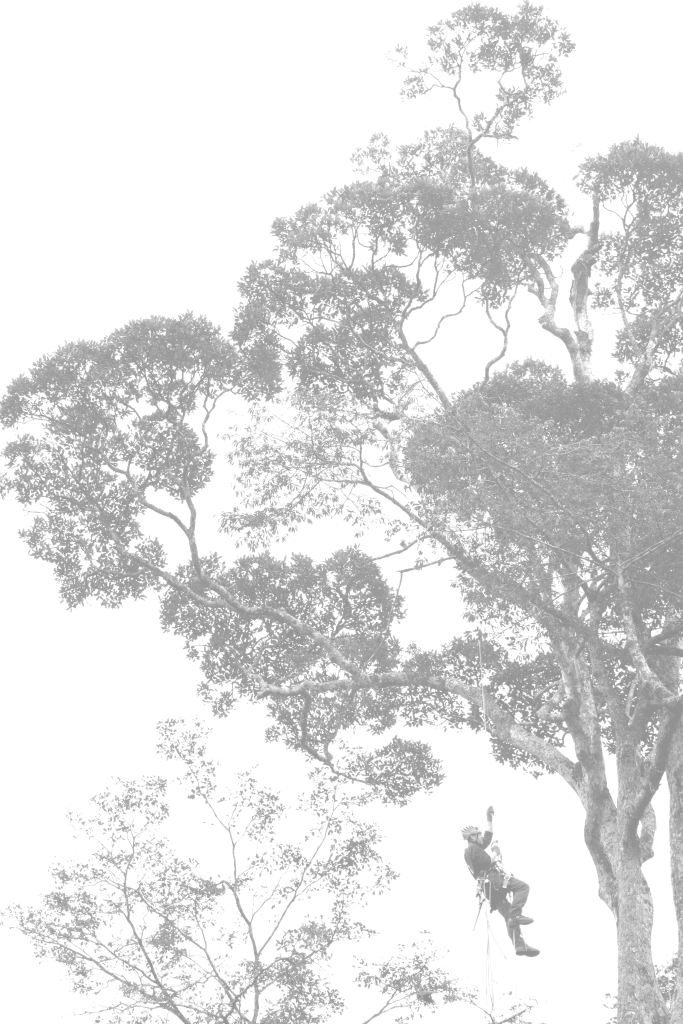
\includegraphics[width=10cm]{Filigrane}
	 \end{textblock}
	\begin{textblock}{140}[0, 1](50, 262)
		\normalfont	Version: \thedate
	\end{textblock}
	\newpage
	~\\ % Print a character or the page will not exist
	\begin{textblock}{140}(40, 40)
		#1
	\end{textblock}
	\begin{textblock}{140}[0,1](40, 270)
		\centering
    \includegraphics[width=5cm]{Logo-Lab}\\ \bigskip
		UMR \'Ecologie des forêts de Guyane\\
		\url{http://www.ecofog.gf}\\[3\baselineskip]
		Les opinions émises par les auteurs sont personnelles et n’engagent ni l’UMR EcoFoG ni ses tutelles.

    \tiny{Photographie en couverture: Hadrien Lalagüe}
	\end{textblock}
	\newpage
}

% PhD / HDR Thesis
%%%%%%%%%%%%%%%%%%%%%%%%%%%%%%%%%%%%%%%%%%%%%%%%%%%%%%%%%%

\usepackage[DocType=PhD, ED=UG, Ets=UG, DIS=ST]{latex/pdgUniv}

\specialty{Écologie}
\defencedate{1er janvier 2018}
\lab{Écologie des Forêts de Guyane}
% ==================
% Setup people like your boss, the jury team and the referees
% - First you need to define how number they will be in each category
%   It is done with the commands \nboss{n}, \nreferee{n} and \njudge{n}.
%   You can define more people in each category than the number given
%   but only the first "\npeople" will be print.
% - Then use the command \makesomeone{<category>}{<number>}{<name>}{<status>}{<other>}
%   where:
%     <category> should be select in ['boss', 'referee', 'judge']
%     <number>   is the rank for printing the person.
%                Only number <= "\npeople" will be printed
%     <name>     First name and las name of the people
%     <status>   Is (s)he a "charg\'e de recher" ou un "professeur d'universit\'e"...
%     <other>    What ever string you want to add (laboratory, jury member place...).
\njudge{7}
\makesomeone{judge}{1}{Prénom NomJury1}{Professeur d'Université}{Membre du Jury}
\makesomeone{judge}{2}{Prénom NomJury2}{Professeur d'Université}{Membre du Jury}
\makesomeone{judge}{3}{Prénom NomJury3}{Professeur d'Université}{Membre du Jury}
\makesomeone{judge}{4}{Prénom NomJury4}{Professeur d'Université}{Membre du Jury}
\makesomeone{judge}{5}{Prénom NomJury5}{Professeur d'Université}{Membre du Jury}
\makesomeone{judge}{6}{Prénom NomJury6}{Professeur d'Université}{Membre du Jury}
\makesomeone{judge}{7}{Prénom NomJury7}{Professeur d'Université}{Membre du Jury}



% End of preamble
%%%%%%%%%%%%%%%%%%%%%%%%%%%%%%%%%%%%%%%%%%%%%%%%%%%%%%%%%%


\begin{document}
\frontmatter

% Title page
%%%%%%%%%%%%%%%%%%%%%%%%%%%%%%%%%%%%%%%%%%%%%%%%%%%%%%%%%%


\makeflyleaf




% Before Body
%%%%%%%%%%%%%%%%%%%%%%%%%%%%%%%%%%%%%%%%%%%%%%%%%%%%%%%%%%




% Contents
%%%%%%%%%%%%%%%%%%%%%%%%%%%%%%%%%%%%%%%%%%%%%%%%%%%%%%%%%%

\LargeMargins
{
\hypersetup{linkcolor=}
\setcounter{tocdepth}{3}
\tableofcontents
}


% Body
%%%%%%%%%%%%%%%%%%%%%%%%%%%%%%%%%%%%%%%%%%%%%%%%%%%%%%%%%%

\LargeMargins
\mainmatter

\chapter{Les forêts tropicales humides, au coeur de l'avenir
planétaire}\label{les-forets-tropicales-humides-au-coeur-de-lavenir-planetaire}

\section{Les écosystèmes forestiers, aujourd'hui
incontournables}\label{les-ecosystemes-forestiers-aujourdhui-incontournables}

Les écosystèmes forestiers correspondent à un assemblage de plantes,
animaux et microorganismes et de leur environnement qui définit une
unité fonctionnelle dont les arbre sont les composants essentiels
\autocite{FRA2000}. Représentant 30\% de la surface globale, ces
écosystèmes sont déterminant dans des enjeux environnementaux, tels que
le maintien du climat, de la biodiversité, et de la qualité de l'eau, de
l'air et des sols, des enjeux économiques, tels que la sécurité
alimentaire et des oportunités de développement ``vert'', et sociaux via
leur valeur patrimoniale. Faire une priorité des forêts dans les
programmes politiques, de recherche et de développement est ainsi
essentiel pour limiter les changements globaux, aller vers un
développement durable de nos sociétés, assurer la sécurité alimentaire
et le bien être des populations \autocites{FRA2015}{Tilman2014}.

Les écosystèmes forestiers accueillent une diversité animale et végétale
et des taux d'endémismes parmi les plus importants du globe
\autocite{Myers2000} et comptent parmi les écosystèmes restés les plus
sauvages \autocite{Mittermeier2003}. Ils représentent de plus niveau
mondial un puits de carbone de 1.1 ± 0.8 Pg C yr\textsuperscript{--1}
\autocite{Pan2011} ce qui en fait un élément clé pour la régulation des
changements globaux et la compensation des émissions gaz à effet de
serre (\emph{GES}) dans l'athmosphère, mais également une importante
source de carbone en cas de diminution des surfaces forestières et
d'émission du carbone stocké dans leur biomasse \autocite{Roy2017}.
Outre leur importance pour la gestion des émissions de GES, les forêts
entretiennent les cycles de l'eau et des nutriments (azote, phosphore,
etc) grâce à leur système racinaire, ce régule la fertilité des sols et
le climat local en maintenant les températures et les précipitations
\autocites{Malhi2008}{Isbell2017}.

Les forêts sont donc parmi les systèmes terrestres les plus riches et en
plus du maintien du climat, du sol, des cycles biogéochimiques majeurs
et de la diversité du vivant. Elles représentent le quotidien des
populations au travers le monde, avec 500 millions de personnes qui en
dépendent directement pour leur subsistance, et sont une source de biens
matériels allant de la nourriture, avec la chasse et la collecte de
produits forestiers non ligneux comestibles, à l'eau, aux matériaux de
construction, et à l'énergie, avec l'utilisationdu bois pour le
chauffage et la cuisson des aliments. Centrale pour l'économie mondiale,
l'exploitation forestière représentait \textasciitilde{} 1\% du PIB et
une part importante de l'emploi au niveau mondial en 2011 et la
dendroénergie est l'une des principales sources d'énergie. Enfin, les
forêts sont interconnectées depuis toujours aux populations humaines et
représentent d'importantes dimensions culturelle, spirituelle et
patrimoniale. \autocites{CBDdiversity2011}{FAO2014}.

\section{Des écosystèmes menacés, en particulier sous les
tropiques}\label{des-ecosystemes-menaces-en-particulier-sous-les-tropiques}

Malgré leur irremplaçable valeur et les multiples biens et services
qu'elles rendent, les écosystèmes forestiers subissent une constante
dégradation, ayant abouti à une perte de 3\% de leur surface globale
entre 2013 et 2015 \autocite{FAO2009}. Les forêts sont en effet soumises
d'une part à de fortes pressions anthropiques, tels que changements
d'usage des terres, introduction d'espèces invasives et exploitation du
bois et de la chasse et d'autre part aux changements globaux qui
provoquent modifications climatiques et athmosphériques et événements
extrêmes de plus en plus fréquents (sécheresses, incendies,
inondations\ldots{}) \autocite{Pachauri2014}. Une prise de conscience
globale, entérinée par la conférence des nations unies sur
l'environnement et le développement tenue à Rio en 1992, a motivé de
nombreuses politiques la surveillance et la conservation de la diversité
et du fonctionnement des forêts
\autocites{Summit1992}{Schlaepfer2000}{Dirzo2003a}{Morales-Hidalgo2015}.
Les pressions exercées sur les forêts et les biens et services
écosystémiques qu'elles rendent se poursuivent malgré tout.

Ce contexte concerne en particulier les forêts tropicales, où les
menaces anthropiques pèsent d'autant plus lourdement que leur rôle est
déterminant au niveau mondial \autocites{Dirzo2003a}{Hansen2013}. Les
bassins forestiers tropicaux représentent 1.3 million d'hectares et
accueillent les plus grandes surfaces de forêts ``primaires'',
\emph{i.e.} forêts anciennes n'ayant pas connu de forte perturbation
anthropique, et représentent les milieux où la diversité biologique est
la plus élevée au monde \autocites{Gentry1988}{FAO2011}. Ces régions de
forêt tropicale, historiquement peu peuplées, connaissent une croissance
démographique de près de 1,4\% par an en moyanne qui soumet les
différents bassins forestiers tropicaux à des pressions croissantes de
chasse, d'exploitation du bois, de conversion en terres agricoles ou de
dégradation en forêts secondaires \autocite{Asner2009}.

Poursuivre les démarches de préservation des forêts et de leur
fonctionnement requiert une attention particulière sur les forêts
tropicales,tout aussi cruciales qu'elles sont aujourd'hui menacées, et
sur une meilleure compréhension de leur fonctionnement et de leur
réponse aux perturbations actuelles.

\section{La biodiversité: clé du fonctionnement des forêts
tropciales}\label{la-biodiversite-cle-du-fonctionnement-des-forets-tropciales}

Les services et processus écosystémiques des forêts dépendent largement
de leur diversité biologique, au sens de la diversité des plantes,
animaux, champignons et microorganismes, de leur variabilité génétique
et phénotypique, et des communautés et écosystèmes qu'ils constituent.
Cette biodiversité garantit une complémentarité entre individus,
permettant d'optimiser l'utilisation des resources naturelles et leur
transformation en biomasse, et qui assure la résilience des écosystèmes
face aux perturbations, aux maladies ou aux invasions. A l'échelle du
globe les forêts tropicales jouent un rôle central de « hotspot » de
biodiversité en abritant près de 50\% des espèces décrites aujourd'hui
\autocite{Wright2005}.

Les menaces qui pèsent sur les écosystèmes forestiers n'épargnent pas
leur diversité biologique menacée par une extinction qualifiée par
certains comme sixième extinction de l'ère moderne
\autocite{Vitousek1997}, d'autant plus inquiétante qu'elle est le seul
changement global réellement irréversible aujourd'hui.

De la grande diversité des forêts tropicales dépend une productivité et
une résilience remarquablement élevées, grâce à la complémentarité des
entre espèces, une utilisation optimale des ressources et une résistance
accrue aux maladies, aux espèces invasives et aux variations
environnementales \autocite{Tilman2014}. L'écologie s'intéresse depuis
longtemps aux patrons de diversité et à leurs déterminants, pour
comprendre d'une part les mécanismes régissant l'assemblage de
différentes espèces en communauté et anticiper leur évolution et leur
réponse à des variations environnementales. A cet égard l'approche
fonctionnelle décrivant les communautés en fonction des caractéristiques
morphologiques, physiologiques et phénologiques des essences qui les
composent \autocite{Violle2007b} semble particulièrement appropriée. La
diversité des communautés est donc représentative de leur fonctionnement
et son étude permet d'appréhender le maintien des processus et services
écosystémiques réalisés par les forêts et d'anticiper leur évolution
dans le contexte de changements globaux et d'exploitation forestière.

\section{Théorie diversité/productivité,
etc}\label{theorie-diversiteproductivite-etc}

Compréhension des mécanismes écologiques, diversité fonctionnelle, lien
avec les cycles étudiés par ailleurs

\section{Impacts des activités anthropiques, intérêts pour la gestion
forestière, contexte Guyanais et tropical en
général}\label{impacts-des-activites-anthropiques-interets-pour-la-gestion-forestiere-contexte-guyanais-et-tropical-en-general}

\chapter{Comment mesurer la diversité biologique
?}\label{comment-mesurer-la-diversite-biologique}

\section{Historique des mesures de
diversité}\label{historique-des-mesures-de-diversite}

\section{Diversité taxonomique}\label{diversite-taxonomique}

\section{Diversité fonctionnelle}\label{diversite-fonctionnelle}

\chapter{L'exemple de Paracou, un site
historique}\label{lexemple-de-paracou-un-site-historique}

\chapter{Problématique et plan de la
thèse}\label{problematique-et-plan-de-la-these}


% Bibliography
%%%%%%%%%%%%%%%%%%%%%%%%%%%%%%%%%%%%%%%%%%%%%%%%%%%%%%%%%%

\backmatter
\SmallMargins

%
\printbibliography


% Tables (of tables, of figures)
%%%%%%%%%%%%%%%%%%%%%%%%%%%%%%%%%%%%%%%%%%%%%%%%%%%%%%%%%%




% After-body (LaTeX code inclusion)
%%%%%%%%%%%%%%%%%%%%%%%%%%%%%%%%%%%%%%%%%%%%%%%%%%%%%%%%%%



% Back cover
%%%%%%%%%%%%%%%%%%%%%%%%%%%%%%%%%%%%%%%%%%%%%%%%%%%%%%%%%%%

% Even page, small margins, no running head, no page number.
\evenpage
\SmallMargins
\thispagestyle{empty}

\begin{normalsize}

\begin{description}

\selectlanguage{french}
\item[Résumé:]
Résumé en Français, en quatrième de couverture.

Lorem ipsum dolor sit amet, consectetuer adipiscing elit. Maecenas
porttitor congue massa. Fusce posuere, magna sed pulvinar ultricies,
purus lectus malesuada libero, sit amet commodo magna eros quis urna.

Nunc viverra imperdiet enim. Fusce est. Vivamus a tellus.

\selectlanguage{french}
\item[Mots clés :]
Mot clé en Français, En liste.
~\\

\selectlanguage{english}
\item[Abstract:]
English abstract, on the last page.

Lorem ipsum dolor sit amet, consectetuer adipiscing elit. Maecenas
porttitor congue massa. Fusce posuere, magna sed pulvinar ultricies,
purus lectus malesuada libero, sit amet commodo magna eros quis urna.

Nunc viverra imperdiet enim. Fusce est. Vivamus a tellus.

\selectlanguage{english}
\item[Keywords:]
Keyword in English, As a list.

\end{description}

\end{normalsize}

\vspace*{\fill}
\centering\includegraphics[width=.3\textwidth]{images/Logo-Lab}
\end{document}
